% **************************************************************************************************
% ** SPSC Report and Thesis Template
% **************************************************************************************************
%
% ***** Authors *****
% Daniel Arnitz, Paul Meissner, Stefan Petrik
% Signal Processing and Speech Communication Laboratory (SPSC)
% Graz University of Technology (TU Graz), Austria
%
% ***** Changelog *****
% 0.1   2010-01-25   extracted from report template by Daniel Arnitz (not ready yet)
% 0.2   2010-02-08   added thesis titlepage and modified layout (not ready yet)
% 0.3   2010-02-18   added TUG logo and statutory declaration
% 0.4   2010-02-18   moved the information fields below % **************************************************************************************************
% ** SPSC Report and Thesis Template
% **************************************************************************************************
%
% ***** Authors *****
% Daniel Arnitz, Paul Meissner, Stefan Petrik
% Signal Processing and Speech Communication Laboratory (SPSC)
% Graz University of Technology (TU Graz), Austria
%
% ***** Changelog *****
%
% ***** Todo *****
%
% **************************************************************************************************



\documentclass[%
a4paper,% !!! ATTENTION: geometry package below !!!
\Twosided,% !!! ATTENTION: geometry package below !!!
openany,% begin chapters with new right page (openright) or don't care (openany)
11pt,%
fleqn,% equations not centered, but on the left side
tablecaptionbelow,% captions below tables
% titlepage,% use title
pointlessnumbers,% do not generate point at the end of section numbers (e.g. 1.4.5 instead of 1.4.5.)
final,%
]{scrreprt}% (KOMA)

\usepackage[paper=a4paper,\Twosided,%
textheight=246mm,%
textwidth=160mm,%
heightrounded=true,% round textheight to multiple of lines (avoids overfull vboxes)
ignoreall=true,% do not include header, footer, and margins in calculations
marginparsep=5pt,% marginpar only used for signs (centered), thus only small sep. needed
marginparwidth=10mm,% prevent margin notes to be out of page
hmarginratio=2:1,% set margin ration (inner:outer for twoside) - (2:3 is default)
]{geometry}%


% master
\usepackage{ifthen}% for optional parts
\usepackage[latin1]{inputenc}% German special characters
\ifthenelse{\equal{\DocumentLanguage}{en}}{\usepackage[USenglish]{babel}}{}%
\ifthenelse{\equal{\DocumentLanguage}{de}}{\usepackage[ngerman]{babel}}{}%
\usepackage[%
headtopline,plainheadtopline,% activate all lines (header and footer)
headsepline,plainheadsepline,%
footsepline,plainfootsepline,%
footbotline,plainfootbotline,%
automark% auto update \..mark
]{scrpage2}% (KOMA)
\usepackage{makeidx}% used to make an index directory
\usepackage[]{caption}% customize captions
\usepackage{multicol}%
\usepackage[stable,bottom,hang,splitrule,multiple,symbol*]{footmisc}% customize footnotes


% text
\usepackage{varioref}% improved references
\usepackage{color}% e.g., for color boxes
\usepackage{rotating}% to rotate objects
\usepackage{gensymb}% symbols (perthousand, Celsius, ...)
\usepackage[right]{eurosym}% euro symbol on the right side (51 EUR)
\usepackage[normalem]{ulem}% cross-out, strike-out, underlines (normalem: keep \emph italic)
%\usepackage[safe]{textcomp}% loading in safe mode to avoid problems (see LaTeX companion)
%\usepackage[geometry,misc]{ifsym}% technical symbols
\usepackage{remreset}%\@removefromreset commands (e.g., for continuous footnote numbering)
\usepackage[%
breaklinks=true,% allow line break in links
colorlinks=true,% if false: framed link
linkcolor=black,anchorcolor=black,citecolor=black,filecolor=black,%
menucolor=black,urlcolor=black]{hyperref}% hyperlinks for references


% math
\usepackage{amsmath,amssymb,amstext,bm} % use math packages
\usepackage{mathcomp}% symbols (perthousand, ...) in math mode


% graphics
\usepackage{graphicx}% use simple graphics
\usepackage{subfigure}% subfigures (a),(b),(c)... within figures
\usepackage{flafter}% place floats always after reference
\usepackage{placeins}% preventing floats from crossing a barrier
\usepackage{float}% to place floats !HERE!
\usepackage{psfrag}% replace text in eps figures


% tables
\usepackage{hhline}% hline doesn't work with colored columns, so using hhline
\usepackage{longtable}% for tables longer than one page
\usepackage{dcolumn}% for number alignment in tables
\usepackage{colortbl}% color in tables


% listings
%\usepackage{alltt}% verbatim environment with commands available
\usepackage{listings}% program code listings


% other
%\usepackage{layout}% graphical page layout (spacings)
\usepackage{xspace}% add space after macros if not followed by punctuation character
\makeindex% used for index creation

 (encoding...)
% 0.5   2010-03-02   added \ShortTitle to fix problems with long thesis titles
%                    added \ThesisType (makes the template suitable for MSc, BSc, PhD, ... Thesis)
%
% ***** Todo *****
% - Introduction/Usage
% **************************************************************************************************

% **************************************************************************************************
% basic setup
\newcommand{\DocumentType}{report} % "thesis" / "report"
\newcommand{\DocumentLanguage}{de} % "en" / "de"
\newcommand{\Twosided}{} % "twoside" / ""


% **************************************************************************************************
% template setup -- do not change these unless you know what you are doing!
% **************************************************************************************************
% ** SPSC Report and Thesis Template
% **************************************************************************************************
%
% ***** Authors *****
% Daniel Arnitz, Paul Meissner, Stefan Petrik
% Signal Processing and Speech Communication Laboratory (SPSC)
% Graz University of Technology (TU Graz), Austria
%
% ***** Changelog *****
%
% ***** Todo *****
%
% **************************************************************************************************



\documentclass[%
a4paper,% !!! ATTENTION: geometry package below !!!
\Twosided,% !!! ATTENTION: geometry package below !!!
openany,% begin chapters with new right page (openright) or don't care (openany)
11pt,%
fleqn,% equations not centered, but on the left side
tablecaptionbelow,% captions below tables
% titlepage,% use title
pointlessnumbers,% do not generate point at the end of section numbers (e.g. 1.4.5 instead of 1.4.5.)
final,%
]{scrreprt}% (KOMA)

\usepackage[paper=a4paper,\Twosided,%
textheight=246mm,%
textwidth=160mm,%
heightrounded=true,% round textheight to multiple of lines (avoids overfull vboxes)
ignoreall=true,% do not include header, footer, and margins in calculations
marginparsep=5pt,% marginpar only used for signs (centered), thus only small sep. needed
marginparwidth=10mm,% prevent margin notes to be out of page
hmarginratio=2:1,% set margin ration (inner:outer for twoside) - (2:3 is default)
]{geometry}%


% master
\usepackage{ifthen}% for optional parts
\usepackage[latin1]{inputenc}% German special characters
\ifthenelse{\equal{\DocumentLanguage}{en}}{\usepackage[USenglish]{babel}}{}%
\ifthenelse{\equal{\DocumentLanguage}{de}}{\usepackage[ngerman]{babel}}{}%
\usepackage[%
headtopline,plainheadtopline,% activate all lines (header and footer)
headsepline,plainheadsepline,%
footsepline,plainfootsepline,%
footbotline,plainfootbotline,%
automark% auto update \..mark
]{scrpage2}% (KOMA)
\usepackage{makeidx}% used to make an index directory
\usepackage[]{caption}% customize captions
\usepackage{multicol}%
\usepackage[stable,bottom,hang,splitrule,multiple,symbol*]{footmisc}% customize footnotes


% text
\usepackage{varioref}% improved references
\usepackage{color}% e.g., for color boxes
\usepackage{rotating}% to rotate objects
\usepackage{gensymb}% symbols (perthousand, Celsius, ...)
\usepackage[right]{eurosym}% euro symbol on the right side (51 EUR)
\usepackage[normalem]{ulem}% cross-out, strike-out, underlines (normalem: keep \emph italic)
%\usepackage[safe]{textcomp}% loading in safe mode to avoid problems (see LaTeX companion)
%\usepackage[geometry,misc]{ifsym}% technical symbols
\usepackage{remreset}%\@removefromreset commands (e.g., for continuous footnote numbering)
\usepackage[%
breaklinks=true,% allow line break in links
colorlinks=true,% if false: framed link
linkcolor=black,anchorcolor=black,citecolor=black,filecolor=black,%
menucolor=black,urlcolor=black]{hyperref}% hyperlinks for references


% math
\usepackage{amsmath,amssymb,amstext,bm} % use math packages
\usepackage{mathcomp}% symbols (perthousand, ...) in math mode


% graphics
\usepackage{graphicx}% use simple graphics
\usepackage{subfigure}% subfigures (a),(b),(c)... within figures
\usepackage{flafter}% place floats always after reference
\usepackage{placeins}% preventing floats from crossing a barrier
\usepackage{float}% to place floats !HERE!
\usepackage{psfrag}% replace text in eps figures


% tables
\usepackage{hhline}% hline doesn't work with colored columns, so using hhline
\usepackage{longtable}% for tables longer than one page
\usepackage{dcolumn}% for number alignment in tables
\usepackage{colortbl}% color in tables


% listings
%\usepackage{alltt}% verbatim environment with commands available
\usepackage{listings}% program code listings


% other
%\usepackage{layout}% graphical page layout (spacings)
\usepackage{xspace}% add space after macros if not followed by punctuation character
\makeindex% used for index creation


\input{./base/layout_\DocumentType}
% **************************************************************************************************
% ** SPSC Report and Thesis Template
% **************************************************************************************************
%
% ***** Authors *****
% Daniel Arnitz, Paul Meissner, Stefan Petrik
% Signal Processing and Speech Communication Laboratory (SPSC)
% Graz University of Technology (TU Graz), Austria
%
% ***** Changelog *****
%
% ***** Todo *****
%
% **************************************************************************************************



% **************************************************************************************************
% * SECTIONING AND TEXT
% **************************************************************************************************

% new chapter, section, ... plus a few addons
%   part
\newcommand{\newpart}[2]{\FloatBarrier\cleardoublepage\part{#1}\label{part:#2}}%
%   chapter
\newcommand{\newchapter}[2]{\FloatBarrier\chapter{#1}\label{chp:#2}}
\newcommand{\newchapterNoTOC}[2]{\FloatBarrier\stepcounter{chapter}\chapter*{#1}\label{chp:#2}}%
%   section
\newcommand{\newsection}[2]{\FloatBarrier\vspace{5mm}\section{#1}\label{sec:#2}}%
\newcommand{\newsectionNoTOC}[2]{\FloatBarrier\vspace{5mm}\stepcounter{section}\section*{#1}\label{sec:#2}}%
%   subsection
\newcommand{\newsubsection}[2]{\FloatBarrier\vspace{3mm}\subsection{#1}\label{sec:#2}}%
\newcommand{\newsubsectionNoTOC}[2]{\FloatBarrier\vspace{3mm}\stepcounter{subsection}\subsection*{#1}\label{sec:#2}}%
%   subsubsection
\newcommand{\newsubsubsection}[2]{\vspace{2mm}\subsubsection{#1}\label{sec:#2}}%
\newcommand{\newsubsubsectionNoTOC}[2]{\vspace{2mm}\stepcounter{subsubsection}\subsubsection*{#1}\label{sec:#2}}%

% next paragraph
\newcommand{\nxtpar}{\par\bigskip}

% "stylish" quotes on the right side
\newcommand{\openingquote}[2]{\hfill\parbox[t]{10cm}{\itshape\raggedleft{"#1"}\\\footnotesize -- #2}\nxtpar}%

% direct quotes
% \newenvironment{directquote}{\nxtpar\hrule}{\hrule}\hfill\litref{#1}{#2}}

% warnings and attention signs in marginpar
\newcommand{\MDanger}{\marginpar{\Huge\centering\fbox{\textbf{!}}}}%
\newcommand{\MAttention}{\marginpar{\Huge\centering\textbf{!}}}%
\newcommand{\MHint}{\marginpar{\Huge\centering\textbf{\checkmark}}}%
\newcommand{\MQuestion}{\marginpar{\Huge\centering\textbf{?}}}%

% same footnote number as last one
\newcommand{\lastfootnotemark}{\addtocounter{footnote}{-1}\footnotemark}%

% value-unit commands (for 457 kHz, etc)
\newcommand{\vu}[2]{\mbox{$#1\,\text{#2}$}} % "value~unit" ... prevents e.g. 456 \linebreak mV
\newcommand{\vuc}[3]{\mbox{$#1\,\text{#2}\;#3\,\%$}} % "value~unit~tolerance-per-cent"
\newcommand{\vum}[3]{\mbox{$#1\,\text{#2}\;#3\,\perthousand$}} % "value~unit~tolerance-per-mil"

% reminders
\newcommand{\reminder}[1]{\colorbox{red}{#1}\xspace}%
\newcommand{\rem}{\reminder{(...)}}%
\newcommand{\remq}{\reminder{???}}%
\newcommand{\uc}{\nxtpar\colorbox{yellow}{... under construction ...}\nxtpar}%

% misc
\newcommand{\pwd}{.} % present working directory (can be used to create relativ paths per part, etc.)


% **************************************************************************************************
% * MATH
% **************************************************************************************************

% highlighting
\newcommand{\vm}[1]{\bm{#1}}% vector or matrix

% operators
\newcommand{\E}[1]{\text{E}\!\left\{#1\right\}}% expectation operator
\newcommand{\var}[1]{\text{var}\!\left\{#1\right\}}% variance operator
\renewcommand{\ln}[1]{\text{ln}\!\left(#1\right)}% natural logarithm
\newcommand{\ld}[1]{\text{ld}\!\left(#1\right)}% logarithm base 2
\renewcommand{\log}[1]{\text{log}\!\left(#1\right)}% logarithm (base 10)
\newcommand{\logb}[2]{\text{log}_{#1}\!\left(#2\right)}% logarithm base ...
\newcommand{\avgvar}[1]{\overline{\text{var}}\!\left\{#1\right\}}% average variance operator
\renewcommand{\Re}[1]{\text{Re}\!\left\{#1\right\}}% real part
\renewcommand{\Im}[1]{\text{Im}\!\left\{#1\right\}}% imaginary part

% other
\newcommand{\conj}{^\ast}% conjugate complex
\newcommand{\mtx}[2]{\left[\begin{array}{#1}#2\end{array}\right]}%vector/matrix


% **************************************************************************************************
% * FLOATS (FIGURES, TABLES, LISTINGS, ...)
% **************************************************************************************************

% figures without frames
%   standard
\newcommand{\fig}[3]{\begin{figure}\centering\includegraphics[width=\textwidth]{#1}\caption{#2}\label{fig:#3}\end{figure}}%
%   with controllable parameters
\newcommand{\figc}[4]{\begin{figure}\centering\includegraphics[#1]{#2}\caption{#3}\label{fig:#4}\end{figure}}%
%   two subfigures
\newcommand{\twofig}[6]{\begin{figure}\centering%
\subfigure[#2]{\includegraphics[width=0.495\textwidth]{#1}}%
\subfigure[#4]{\includegraphics[width=0.495\textwidth]{#3}}%
\caption{#5}\label{fig:#6}\end{figure}}%
%   two subfigures and controllable parameters
\newcommand{\twofigc}[8]{\begin{figure}\centering%
\subfigure[#3]{\includegraphics[#1]{#2}}%
\subfigure[#6]{\includegraphics[#4]{#5}}%
\caption{#7}\label{fig:#8}\end{figure}}%

% framed figures
%   standard
\newcommand{\figf}[3]{\begin{figure}\centering\fbox{\includegraphics[width=\textwidth]{#1}}\caption{#2}\label{fig:#3}\end{figure}}%
%   with controllable parameters
\newcommand{\figcf}[4]{\begin{figure}\centering\fbox{\includegraphics[#1]{#2}}\caption{#3}\label{fig:#4}\end{figure}}%
%   two subfigures
\newcommand{\twofigf}[6]{\begin{figure}\centering%
\fbox{\subfigure[#2]{\includegraphics[width=0.495\textwidth]{#1}}}%
\fbox{\subfigure[#4]{\includegraphics[width=0.495\textwidth]{#3}}}%
\caption{#5}\label{fig:#6}\end{figure}}%
%   two subfigures and controllable parameters
\newcommand{\twofigcf}[8]{\begin{figure}\centering%
\fbox{\subfigure[#3]{\includegraphics[#1]{#2}}}%
\fbox{\subfigure[#6]{\includegraphics[#4]{#5}}}%
\caption{#7}\label{fig:#8}\end{figure}}%

% listings
\newcommand{\filelisting}[4]{\lstinputlisting[print=true,language=#1,caption={#3},label={lst:#4}]{#2}}

% preserve backslash for linebreaks in tables (ragged... redefines \\, thus it has to be preserved)
\newcommand{\pbs}[1]{\let\temp=\\#1\let\\=\temp}%

\graphicspath{{./drawings/}{./plots/}{./images/}}
% **************************************************************************************************
% ATTENTION: Make sure that makeindex is set to -s "./base/index.sty"
% **************************************************************************************************

% uncomment to get watermarks:
% \usepackage[first,bottom,light,draft]{draftcopy}
% \draftcopyName{ENTWURF}{160}


% **************************************************************************************************
% information fields

% general
\newcommand{\DocumentTitle}{Adaptive Systems}
\newcommand{\DocumentSubtitle}{Assignment 2}
\newcommand{\ShortTitle}{Assignment 2} % used in headers (keep short!)
\newcommand{\DocumentAuthor}{Ebner Thomas (0831246), N�hmer Stefan (0830668)}
\newcommand{\DocumentDate}{Graz, \today}
%    for thesis only (will be ignored for reports)
\newcommand{\ThesisType}{Master's Thesis}
\newcommand{\Organizations}{Signal Processing and Speech Communications Laboratory \\ Graz University of Technology \\[1cm] on behalf of \\ Some Company} % SPSC \\ TUG \\[1cm] on behalf of \\ A Nice Company
\newcommand{\Advisors}{Dipl.-Ing. Dr. Assoc.Prof. Klaus Witrisal \\ Dipl.-Ing. Paul Meissner} % Advisor 1 \\ Advisor 2 \\ ...
\newcommand{\Supervisors}{Univ.-Prof. Dipl.-Ing. Dr.techn. Gernot Kubin}

% revision number
\newcommand{\RevPrefix}{alpha~}
\newcommand{\RevLarge}{1}
\newcommand{\RevSmall}{0}

% confidential?
\newcommand{\ConfidNote}{do not blend}% {"confidential", "eyes only", ...}





\begin{document}

%listingstyle:
\definecolor{orange}{rgb}{0.75,0.65,0}
\definecolor{gruen}{rgb}{0,0.5,0}
\definecolor{listinggray}{gray}{0.97}
\definecolor{listingshadow}{gray}{0.2}
\lstloadlanguages{Matlab}
\lstset{frame=shadowbox,
		rulesepcolor=\color{listingshadow},
		numbers=left,
		basicstyle=\scriptsize\ttfamily,
		numberstyle=\tiny,
		keywordstyle=\color{blue}\bfseries, % bold black keywords
		identifierstyle=, % nothing happens
		commentstyle=\color{gruen}, % comments
		stringstyle=\color{orange}, % typewriter type for strings
		showstringspaces=false,
		tabsize=4,
		backgroundcolor=\color{listinggray}
        }




% **************************************************************************************************
% titlepage
\input{./base/titlepage_\DocumentType}

% statutory declaration for theses
\ifthenelse{\equal{\DocumentType}{thesis}}{% **************************************************************************************************
% ** SPSC Report and Thesis Template
% **************************************************************************************************
%
% ***** Authors *****
% Daniel Arnitz, Paul Meissner, Andreas Laesser, Stefan Petrik
% Signal Processing and Speech Communication Laboratory (SPSC)
% Graz University of Technology (TU Graz), Austria
%
% ***** Changelog *****
% 0.1   2010-02-18   created
% 0.2   2010-03-02   added German declaration
%
% ***** Todo *****
% **************************************************************************************************

\cleardoublepage
\pagestyle{empty}\pagenumbering{roman}

\vspace*{1cm}

% English
\ifthenelse{\equal{\DocumentLanguage}{en}}{
\begin{center}\Large\bfseries Statutory Declaration\end{center}\vspace*{1cm}
\noindent I declare that I have authored this thesis independently, that I have not used other than the declared sources$/$resources, and that I have explicitly marked all material which has been quoted either literally or by content from the used sources.
\par\vspace*{4cm}
\centerline{
\begin{tabular}{m{1.5cm}cm{1.5cm}m{3cm}m{1.5cm}cm{1.5cm}}
\cline{1-3} \cline{5-7}
 & date & & & & (signature) &\\
\end{tabular}}
}

% German
\ifthenelse{\equal{\DocumentLanguage}{de}}{
\begin{center}\Large\bfseries Eidesstattliche Erkl�rung\end{center}\vspace*{1cm}
Ich erkl�re an Eides statt, dass ich die vorliegende Arbeit selbstst�ndig verfasst, andere als die angegebenen Quellen$/$Hilfsmittel nicht benutzt, und die den benutzten Quellen w�rtlich und inhaltlich entnommene Stellen als solche kenntlich gemacht habe.
\par\vspace*{4cm}
\centerline{
\begin{tabular}{m{1.5cm}cm{1.5cm}m{3cm}m{1.5cm}cm{1.5cm}}
\cline{1-3} \cline{5-7}
 & Graz, am & & & & (Unterschrift) &\\
\end{tabular}}
}

}{}


% **************************************************************************************************
% **************************************************************************************************
% user-defined part

\chapter{MATLAB Problem 2.1}

In den Abbildungen \ref{fig:2_1_noisefree} bis \ref{fig:2_1_noise_norm} sind die Filterkoeffizienten des
Adaptiven Filters dargestellt. Beim rauschfreien Fall in Abbildung \ref{fig:2_1_noisefree} erkennt man,
dass der Adaptive Filter die Koeffizienten des unbekannten Systems sehr schnell ann�hert. Da kein Rauschen
hinzugef�gt wird, werden diese Koeffizienten sehr gut angeh�hert.

In den Abbiludungen \ref{fig:2_1_noise} und \ref{fig:2_1_noise_norm} ist sehr gut der Unterschied zwischen
NLMS und LMS zu erkennen.

Beim LMS n�hern sich die Koeffizienten etwas schneller als beim NLMS an. Der Grund hierf�r ist, dass beim NLMS
$\mu$ durch der Norm des tapped input Vektors angepasst wird. Bei einer Varianz des Eingangssignals (white noise) von $1$
und einer Filterordnung von 4, wird $\mu$ im Mittel durch 4 dividiert.

Durch das kleinere errektive $\mu$ n�hert sich der NLMS etwas langsamer den Koeffizienten an. Allerdings ist durch das 
kleinere $\mu$ der Excess-Error kleiner (siehe Vorlesung vom 18.11). Somit enthalten die Koeffizienten weniger Fluktuation (weniger Rauschen).
Die Abbildungen \ref{fig:2_1_noise} und \ref{fig:2_1_noise_norm} schildern sehr gut die geschilderten
zusammenh�nge wieder.
\begin{figure}[ht!]
 \centering
 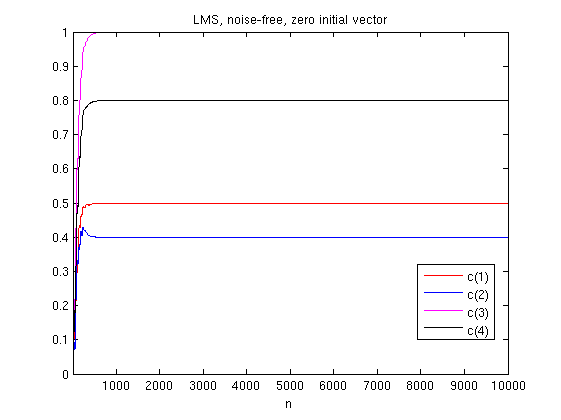
\includegraphics[width=12cm]{./plots/2_1_noisefree.png}
 % 2_3_a_0_0001.png: 560x420 pixel, 90dpi, 15.81x11.85 cm, bb=
 \caption{LMS, $\mu=0.01$, zero-mean white noise input signal with unit variance}
 \label{fig:2_1_noisefree}
\end{figure}


\begin{figure}[ht!]
 \centering
 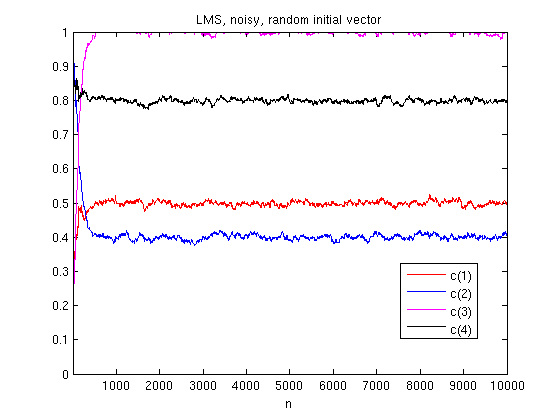
\includegraphics[width=12cm]{./plots/2_1_noise.png}
 % 2_3_a_0_0001.png: 560x420 pixel, 90dpi, 15.81x11.85 cm, bb=
 \caption{LMS, $\mu=0.01$, zero-mean white noise input signal with unit variance, and additional white noise}
 \label{fig:2_1_noise}
\end{figure}


\begin{figure}[ht!]
 \centering
 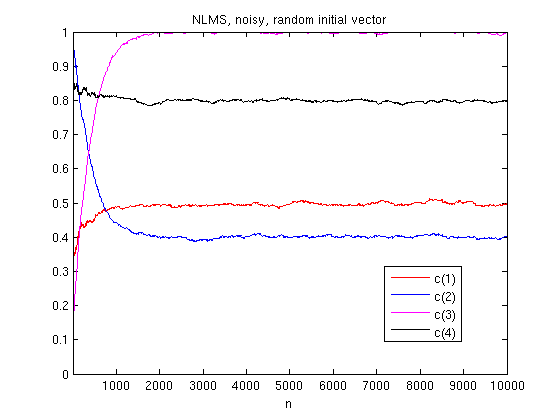
\includegraphics[width=12cm]{./plots/2_1_noise_norm.png}
 % 2_3_a_0_0001.png: 560x420 pixel, 90dpi, 15.81x11.85 cm, bb=
 \caption{NLMS, $\mu=0.01$, zero-mean white noise input signal with unit variance, and additional white noise}
 \label{fig:2_1_noise_norm}
\end{figure}
\clearpage
\chapter{Analytic Problem 1.2}

\paragraph{a)}
Wie in der "Ubung om 25.10.2011 Hergeleitet kann die Kostenfunktion wie folgt angeschrieben werden:

\begin{equation}
 J(\vm{c}) = \sigma_v^2 - 2\vm{c}^T \vm{p} + \vm{c}^T\vm{R}_{xx}\vm{c}
\label{eq:cost1}
\end{equation}

Die Gleichung \ref{eq:cost1} kann wie folgt umformuliert werden:

\begin{equation}
 J(\vm{c}) = \sigma_v^2 - \vm{p}^T\vm{R}_{xx}^{-1}\vm{p} + (\vm{c} - \vm{R}_{xx}^{-1}\vm{p})^T\vm{R}_{xx}(\vm{c} - \vm{R}_{xx}^{-1}\vm{p})
\label{eq:cost2}
\end{equation}


Beweis: Durch Ausmultiplizieren der Klammern gelangt man wieder auf die Gleichung \ref{eq:cost1}:

\begin{align}
 J(\vm{c}) &= \sigma_v^2 - \vm{p}^T\vm{R}_{xx}^{-1}\vm{p} + (\vm{c}^T - \vm{p}\vm{R}_{xx}^{-1})(\vm{R}_{xx}\vm{c} - \vm{R}_{xx}\vm{R}_{xx}^{-1}\vm{p}) \\
  &=  \sigma_v^2 - \vm{p}^T\vm{R}_{xx}^{-1}\vm{p} + \vm{c}^T\vm{R}_{xx}\vm{c} - \vm{p}^T\vm{R}_{xx}^{-1}\vm{R}_{xx}\vm{c} - \vm{c}^T\vm{p} + \vm{p}^T\vm{R}_{xx}^{-1}\vm{p} \\
  &=  \sigma_v^2 + \vm{c}^T\vm{R}_{xx}\vm{c} - \vm{p}^T\vm{c} - \vm{c}^T\vm{p} \\
  &=  \sigma_v^2 + \vm{c}^T\vm{R}_{xx}\vm{c} - 2 \vm{c}^T\vm{p}
\label{eq:cost_beweis}
\end{align}

In der Gleichung \ref{eq:cost2} kommt der Ausdruck $\vm{c} - \vm{R}_{xx}^{-1}\vm{p}$ vor. Dieser Ausdruck entspricht
genau dem Misalignment-Vector, da $\vm{R}_{xx}^{-1}\vm{p}$ der Wiener Hopf-Solution entspricht und somit die optimale
L"osung darstellt.

Somit kann die Kostenfunktion in Abh"angigkeit von $\vm{v}$ (Misalignment-Vektor) ausgedr"uckt werden:
\begin{equation}
 J(\vm{c}) = \sigma_v^2 - \vm{p}^T\vm{R}_{xx}^{-1}\vm{p} + \vm{v}^T\vm{R}_{xx}\vm{v}
\label{eq:cost3}
\end{equation}
Anhand dieser Gleichung erkennt man, dass der vordere Teil ($\sigma_v^2 - \vm{p}^T\vm{R}_{xx}^{-1}\vm{p}$)
unabh"angig vom Misalignment-Vektor ist und somit das Minimum der Kostenfunktion($J_{min}$) darstellt.

\paragraph{b)}

Die Autokorrelationsmatrix $\vm{R}_{xx}$ kann mittels der Eigenwerte/Eigenvektoren wie folgt zerlegt werden:

\begin{equation}
\vm{R}_{xx} = \vm{Q}\vm{\Delta}\vm{Q}^T
\end{equation}

Wobei die Matrix $\vm{\Delta}$ eine Diagonalmatrix ist, welche die Eigenwerte von $\vm{R}_{xx}$ enth"alt.
Die Matrix $\vm{Q}$ enth"alt alle Eigenvektoren.

Diese Beziehung kann in die Gleichung \ref{eq:cost3} eingesetzt werden und man erh"alt:

\begin{equation}
 J(\vm{c}) = J_{min} + \vm{v}^T\vm{Q}\vm{\Delta}\vm{Q}^T\vm{v}
\label{eq:costasfd}
\end{equation}

F"ugt man nun noch folgende Substituion ein: $\vm{\tilde{v}} = \vm{Q}^T\vm{v}$, so erh"alt man
eine Gleichung f"ur die Kostenfunktion bei der die einzelnen Komponenten von $\vm{\tilde{v}}$ entkoppelt sind:

\begin{equation}
 J(\vm{c}) = J_{min} + \vm{\tilde{v}}^T\vm{\Delta}\vm{\tilde{v}}
\label{eq:cost4}
\end{equation}

Die Gleichung \ref{eq:cost4} in Matrixschreibweise kann nun wie folgt in eine Summe umgeschrieben werden:

\begin{equation}
 J(\vm{c}) = J_{min} + \sum_{k=1}^N \tilde{v}_k^2 \lambda_k
\label{eq:cost5}
\end{equation}

\paragraph{c)}

Wie in der "Ubung vom 22.11.2011 gezeit wurde, verhalten sich die einzelnen Komponenten von $\vm{\tilde{v}}$
wie folgt:

\begin{equation}
 \tilde{v}_k[n] = (1-\mu \lambda_k)^n \tilde{v}_k[0] = \tilde{v}_k[0]e^{-n/\tau_k}
\label{eq:misalignment_evolution}
\end{equation}

Diese Gleichung in Gleichung \ref{eq:cost5} eingesetzt ergibt:
\begin{equation}
 J(\vm{c}) = J_{min} + \sum_{k=1}^N \tilde{v}_k^2[0] \lambda_k e^{-2n/\tau_k}
\label{eq:cost6}
\end{equation}

\paragraph{d)}

Die Zeitkonstanten k"onnen aus der Gleichung \ref{eq:misalignment_evolution} ermittelt werden:
Daraus ergibt sich f"ur $\tau_k$ (wie auch in der "Ubung bereits hergeleitet) folgendes:

\begin{equation}
 \tau_k = \frac{-1}{log|1-\mu \lambda_k|}  \approx \frac{1}{\mu \lambda_k}
\end{equation}

\begin{equation}
 J(\vm{c}) = J_{min} + \sum_{k=1}^N \tilde{v}_k^2[0] \lambda_k e^{-2n \mu \lambda_k}
\label{eq:cost7}
\end{equation}

\paragraph{e)}

White noise with unit variance => $R_{xx} = \vm{I}$. Die Eigenenwerte einer Diagonalmatrix entsprechen genau
den Werten in der Diagonale. Somit sind beide Eigenwerte = 1.
Die Eigenvektoren sind $[1 0]^T$ und $[0 1]^T$. Die Eigenvektoren in die Matrix $\vm{Q}$ eingetragen ergibt:

\begin{equation}
 \vm{Q}^T = \vm{Q} = \begin{pmatrix} 1 & 0 \\ 0 & 1 \end{pmatrix}
\end{equation}

\begin{equation}
 \vm{\tilde{v}}[0] = \vm{Q}^T \vm{v}[0] = \begin{pmatrix} -2 \\ -1 \end{pmatrix}
\end{equation}

Diese Werte in die Gleichung f"ur die Kostenfunktion eingesetzt ergibt:

\begin{equation}
 J(\vm{c}) = J_{min} + 4e^{-2n\mu} + e^{-2n\mu}
\label{eq:cost_example}
\end{equation}
\clearpage
\chapter{MATLAB Problem 2.3}

\paragraph{a)}

In den Plots ist deutlich ersichtlich, dass $\mu$ direkt in die Zeitkonstanten, also in die
Konvergenzgeschwindigkeit einflie�t. Im Falle von zero-mean White-Noise sind alle Eigenwerte der
Autokorrelationsmatrix 1. Somit ergeben sich die Zeitkonstanten theoretisch: $\approx \frac{1}{\mu \lambda_k} = \frac{1}{\mu}$.
Diese Formel stimmte auch sehr gut mit den aus den Plots ermittelten Werten f�r $\tau_k$ �berein.
Wie in der Abbildung \ref{fig:2_3_a_1} zu sehen, ist der Algorithmus bei $\mu=1$ im Falle des LMS instabil.
Der Misalignmentvector divergiert und der MSE wird immer gr��er.
Beim NLMS und $\mu=1$ ist keine deutliche Konvergenz des Misalignmentvectors ersichtlich. Der Misalignmentvector
divergiert allerdings auch nicht so wie beim LMS(ohne Normalisierung). Der Grund hierf�r ist, dass $\mu$ durch
$\vm{x}[n]$ dividiert wird und somit etwas kleiner ist. $\mu$ ist aber dennoch zu gro� um die Koeffizienten vern�nftig
anzun�hern.


F�r ein gr��eres $\mu$ konvergiert der MSE wesentlich schneller gegen sein Minimum, allerdings ist auch
der Excess-Error etwas gr��er.

Beim NLMS wird $\mu$ durch $|\vm{x}[n]|^2$ dividiert. Bei einer Varianz von 1 und einer Filterordnung $N=3$ ist
der tapped input Vektor $\vm{x}[n]$ 3 Elemente gro�. Somit ergibt sich ein Erwartungswert f�r $\vm{x}[n]$ von 3.
Aus diesem Grund sind die Zeitkonstanten f�r diese Eingangsvarianz um den Faktor 3 gr��er. Der entscheidende Vorteil
beim LMS ist jetzt, dass die Konvergenzgeschwindigkeit nicht mehr von der Eingangsvarianz abh�ngt. Diese
ist im n�chsten Abschnitt zu sehen.

\begin{figure}[ht!]
 \centering
 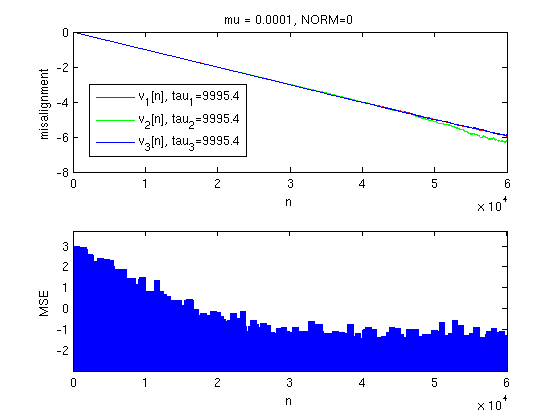
\includegraphics[width=12cm]{./plots/2_3_a_0_0001.png}
 % 2_3_a_0_0001.png: 560x420 pixel, 90dpi, 15.81x11.85 cm, bb=
 \caption{LMS, $\mu=0.0001$, zero-mean unit variance white noise input}
 \label{fig:2_3_a_0_0001}
\end{figure}

\begin{figure}[ht!]
 \centering
 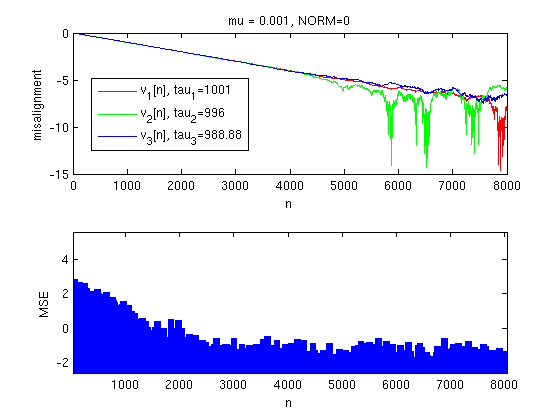
\includegraphics[width=12cm]{./plots/2_3_a_0_001.png}
 % 2_3_a_0_0001.png: 560x420 pixel, 90dpi, 15.81x11.85 cm, bb=
 \caption{LMS, $\mu=0.001$, zero-mean unit variance white noise input}
 \label{fig:2_3_a_0_001}
\end{figure}

\begin{figure}[ht!]
 \centering
 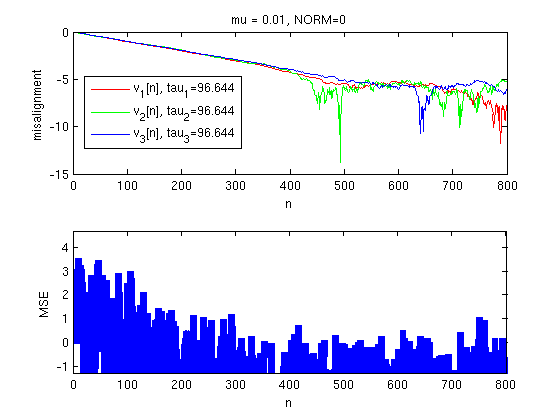
\includegraphics[width=12cm]{./plots/2_3_a_0_01.png}
 % 2_3_a_0_0001.png: 560x420 pixel, 90dpi, 15.81x11.85 cm, bb=
 \caption{LMS, $\mu=0.01$, zero-mean unit variance white noise input}
 \label{fig:2_3_a_0_01}
\end{figure}

\begin{figure}[ht!]
 \centering
 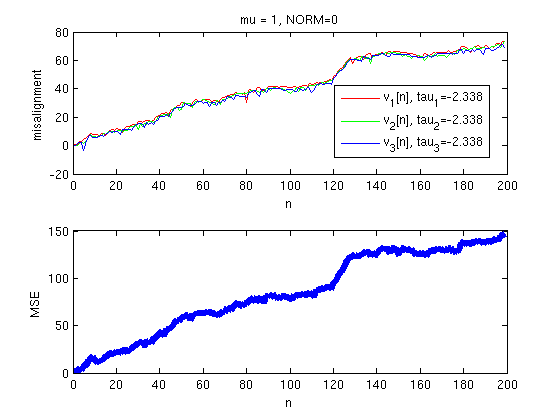
\includegraphics[width=12cm]{./plots/2_3_a_1.png}
 % 2_3_a_0_0001.png: 560x420 pixel, 90dpi, 15.81x11.85 cm, bb=
 \caption{LMS, $\mu=1$, zero-mean unit variance white noise input}
 \label{fig:2_3_a_1}
\end{figure}

%NLMS:
\begin{figure}[ht!]
 \centering
 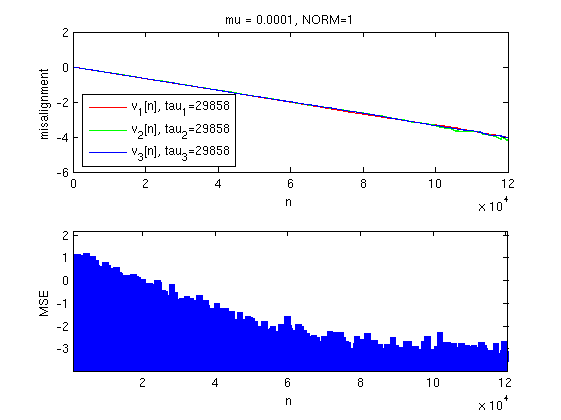
\includegraphics[width=12cm]{./plots/2_3_a_0_0001_norm.png}
 % 2_3_a_0_0001.png: 560x420 pixel, 90dpi, 15.81x11.85 cm, bb=
 \caption{NLMS, $\mu=0.0001$, zero-mean unit variance white noise input}
 \label{fig:2_3_a_0_0001_norm}
\end{figure}

\begin{figure}[ht!]
 \centering
 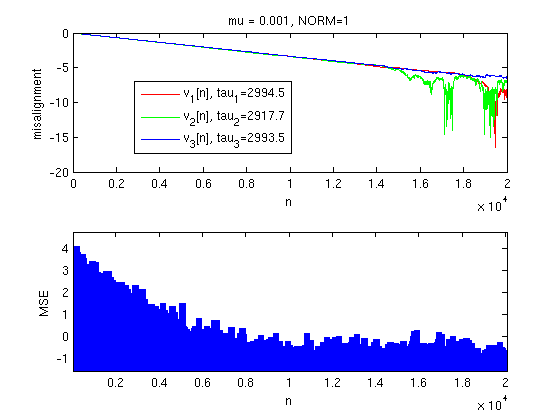
\includegraphics[width=12cm]{./plots/2_3_a_0_001_norm.png}
 % 2_3_a_0_0001.png: 560x420 pixel, 90dpi, 15.81x11.85 cm, bb=
 \caption{NLMS, $\mu=0.001$, zero-mean unit variance white noise input}
 \label{fig:2_3_a_0_001_norm}
\end{figure}

\begin{figure}[ht!]
 \centering
 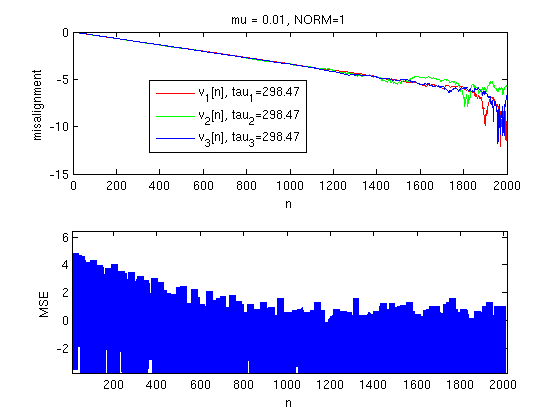
\includegraphics[width=12cm]{./plots/2_3_a_0_01_norm.png}
 % 2_3_a_0_0001.png: 560x420 pixel, 90dpi, 15.81x11.85 cm, bb=
 \caption{NLMS, $\mu=0.01$, zero-mean unit variance white noise input}
 \label{fig:2_3_a_0_01_norm}
\end{figure}

\begin{figure}[ht!]
 \centering
 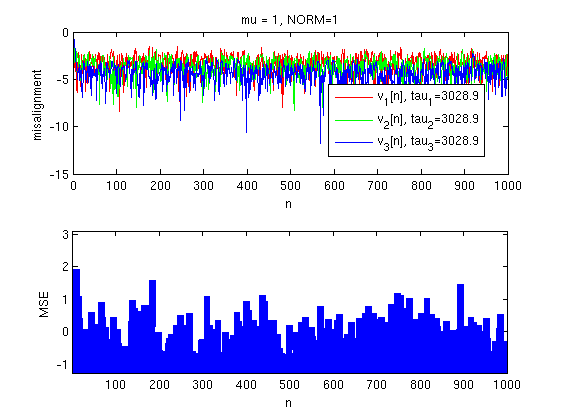
\includegraphics[width=12cm]{./plots/2_3_a_1_norm.png}
 % 2_3_a_0_0001.png: 560x420 pixel, 90dpi, 15.81x11.85 cm, bb=
 \caption{NLMS, $\mu=1$, zero-mean unit variance white noise input}
 \label{fig:2_3_a_1_norm}
\end{figure}

\clearpage

\paragraph{b)}

In den Plots wird ersichtlich, dass die Konvergenzgeschwindigkeit des LMS von der Varianz des Eingangssingals
abh�ngt. Somit Konvergiert dieser Algorithmus bei einer gr��eren Varianz von $\vm{x}[n]$ schneller, bzw. bei einer
sehr geringen Eingangsvarianz nur sehr gering. Um das ganze noch mit zahlen zu belegen, betrachten wir zun�chst
wieder die Formel f�r die Zeitkonstanten: $\tau_k \approx \frac{1}{\mu \lambda_k}$. Da es sich wieder um
wei�es Rauschen handelt, sind alle Eigenwerte $\lambda_k$ gleich und entsprechen der Varianz.
Somit ergibt sich bei einer Eingangsvarianz von $1.5$ theoretisch eine Zeitkonstante von $1/(1.5\mu) \approx 0.666/\mu$.
Diese Werte k�nnen sehr gut anhand der Plots abgelesen werden.

Beim NLMS hat die Eingangsvarianz keinen Einfluss da $\mu$ entsprechend der Eingangsvarianz angepasst wird.
Dies ist sehr gut anhand der berechneten Zeitkonstanten in den Abbildungen \ref{fig:2_3_b_xvar_0_2_norm} und \ref{fig:2_3_b_xvar_1_5_norm}
zu sehen.

\begin{figure}[ht!]
 \centering
 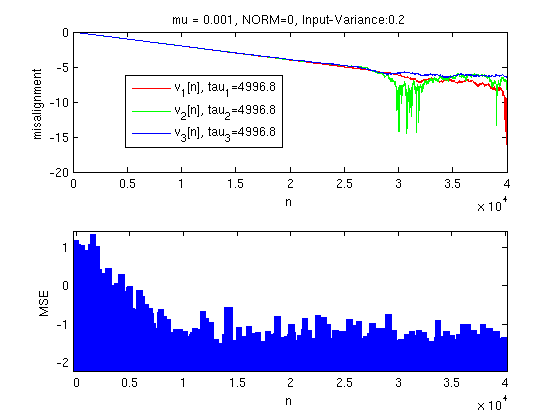
\includegraphics[width=12cm]{./plots/2_3_b_xvar_0_2.png}
 % 2_3_a_0_0001.png: 560x420 pixel, 90dpi, 15.81x11.85 cm, bb=
 \caption{LMS, $\mu=0.001$, zero-mean white noise input with variance=$0.2$}
 \label{fig:2_3_b_xvar_0_2}
\end{figure}

\begin{figure}[ht!]
 \centering
 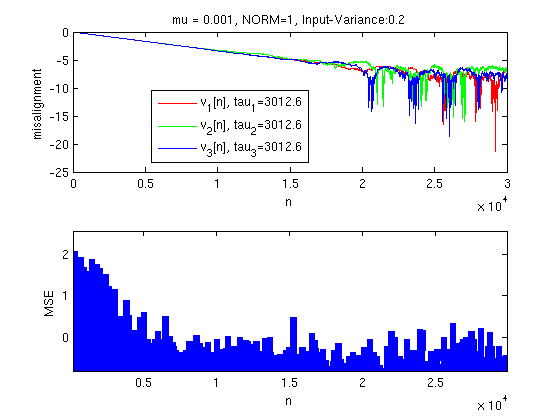
\includegraphics[width=12cm]{./plots/2_3_b_xvar_0_2_norm.png}
 % 2_3_a_0_0001.png: 560x420 pixel, 90dpi, 15.81x11.85 cm, bb=
 \caption{NLMS, $\mu=0.001$, zero-mean white noise input with variance=$0.2$}
 \label{fig:2_3_b_xvar_0_2_norm}
\end{figure}

\begin{figure}[ht!]
 \centering
 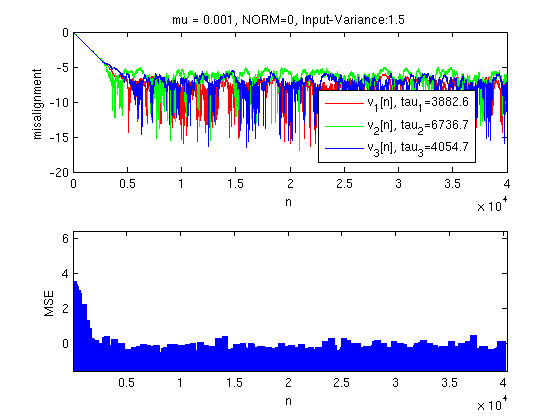
\includegraphics[width=12cm]{./plots/2_3_b_xvar_1_5.png}
 % 2_3_a_0_0001.png: 560x420 pixel, 90dpi, 15.81x11.85 cm, bb=
 \caption{LMS, $\mu=0.001$, zero-mean white noise input with variance=$1.5$}
 \label{fig:2_3_b_xvar_1_5}
\end{figure}

\begin{figure}[ht!]
 \centering
 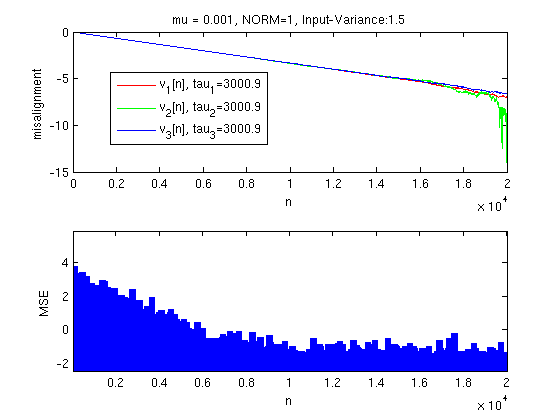
\includegraphics[width=12cm]{./plots/2_3_b_xvar_1_5_norm.png}
 % 2_3_a_0_0001.png: 560x420 pixel, 90dpi, 15.81x11.85 cm, bb=
 \caption{NLMS, $\mu=0.001$, zero-mean white noise input with variance=$1.5$}
 \label{fig:2_3_b_xvar_1_5_norm}
\end{figure}


\paragraph{c)}

Da das Eingangssignal jetzt kein Wei�es Rauschen mehr ist, sind die Eigenwerte von $\vm{R}_{xx}$ nicht mehr gleich.
Dadurch konvergieren die Komponenten von $v$ unterschiedlich schnell.

Der MSE nimmt kontinuierlich ab, bis er den noise-floor erreicht (MMSE + excess-error).

\begin{figure}[ht!]
 \centering
 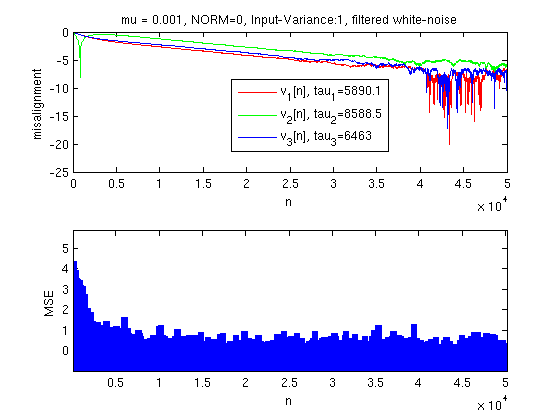
\includegraphics[width=12cm]{./plots/2_3_c.png}
 % 2_3_a_0_0001.png: 560x420 pixel, 90dpi, 15.81x11.85 cm, bb=
 \caption{LMS, $\mu=0.001$, zero-mean white noise input with variance=$1$, filtered}
 \label{fig:2_3_c}
\end{figure}

\begin{figure}[ht!]
 \centering
 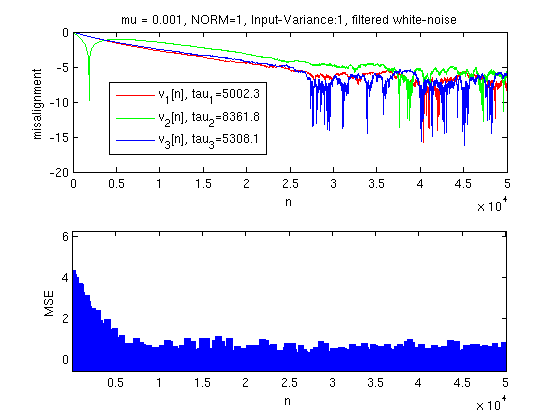
\includegraphics[width=12cm]{./plots/2_3_c_norm.png}
 % 2_3_a_0_0001.png: 560x420 pixel, 90dpi, 15.81x11.85 cm, bb=
 \caption{NLMS, $\mu=0.001$, zero-mean white noise input with variance=$1$, filtered}
 \label{fig:2_3_c}
\end{figure}

\clearpage
\paragraph{d)}
Der MSE nimmt kontinuierlich ab, bis er den noise-floor erreicht (MMSE + excess-error).

\paragraph{e)}

Berechnung des Excess Errors:
Wie in der Vorlesung vom 18.11.2011 hergeleitet ergibt sich der Excess Error wie folgt:

\begin{equation}
 M \cdot MMSE
\end{equation}

Wobei $M$ als Misadjustment bezeichnet wird

\begin{equation}
 M = \frac{\mu ||\vm{x[n]}||^2}{2-\mu ||\vm{x[n]}||^2}
\end{equation}
Wobei $\vm{x[n]}||^2$ Der Varianz des Eingangssingals entspricht.

Das Minimum der Kostenfunktion(=MMSE) (siehe Gleichung \ref{eq:cost3} wurde wie folgt ermittelt:

\begin{equation}
MMSE = \sigma_v^2 - \vm{p}^T\vm{R}_{xx}^{-1}\vm{p}
\label{eq:bla}
\end{equation}

Formt man nun die Wiener Hopf Solution auf $\vm{p}$ um so erh�lt man:
$\vm{p} = \vm{R}_{xx}\vm{h}$. In die Gleichung \ref{eq:bla} eingesetzt ergibt das (f"ur white noise!!!):

\begin{equation}
MMSE = \sigma_v^2 - \vm{h}^T\vm{R}_{xx}^T \vm{R}_{xx}^{-1} \vm{R}_{xx}\vm{h} = \sigma_v^2 -\vm{h}^T\vm{R}_{xx}^T\vm{h}
= \sigma_v^2 - ||h||\sigma_x^2
\label{eq:bla1}
\end{equation}

\begin{equation}
 excess error = MMSE \cdot M
\end{equation}


Nun ergeben sich folgende Werte f�r den Excesserror in dB:\\


\begin{table}[!htp]
\begin{center}
\begin{tabular}
{| c || c | c | c | c | c |}   %  || zur Unterteilung eingestellte/gemnessene/berechnete Werte
\hline
Eingangs-Varianz $\sigma_x^2$ & $\mu = 0.0001$ & $\mu = 0.001$ & $\mu = 0.01$ & $\mu = 1$ \\ \hline \hline
1 & -44.31 & -34.31 & -24.31 & -4.31 \\ \hline
1.5 &  -40.7786 & -30.7786 & -20.7786 &  -0.7786 \\ \hline
0.2 & -58.4873 & -48.4873 & -38.4873 & -18.4873 \\ \hline
\end{tabular}
\caption{Ermittelten Werte f�r den Excess-Error in dB beim LMS}
\end{center}
\end{table}

\begin{table}[!htp]
\begin{center}
\begin{tabular}
{| c || c | c | c | c | c |}   %  || zur Unterteilung eingestellte/gemnessene/berechnete Werte
\hline
Eingangs-Varianz $\sigma_x^2$ & $\mu = 0.0001$ & $\mu = 0.001$ & $\mu = 0.01$ & $\mu = 1$ \\ \hline \hline
1 & -49.0873 & -39.0873 & -29.0873  & -9.0873 \\ \hline
1.5 &  -45.5498 & -35.5498 & -25.5498 &  -5.5498 \\ \hline
0.2 & -63.2585 & -53.2585 & -43.2585 & -23.2585 \\ \hline
\end{tabular}
\caption{Ermittelten Werte f�r den Excess-Error in dB beim NLMS}
\end{center}
\end{table}

Wie bereits erkl"art nimmt der Excesserror bei einem kleinerem $\mu$ ab. Bei einer kleineren Eingangsvarianz
ist der Excesserror auch kleiner. Da beim NLMS das effektive $\mu$ verkleinert wird, ist bei dieser Variante des
LMS der Excesserror etwas geringer.

\clearpage


\section{Analytical Problem 2.4: Average Behaviour of the LMS}

Zur Berechnung wurde die Struktur aus Abbildung 2 in der Angabe verwendet. Das Eingangssignal $x[n]$ ist \emph{white}, laut der Angabe zur Abbildung 2 ist das Noise $\nu[n]$ ebenfalls \emph{white Gaussian noise}, die beiden sind also nicht korreliert und \emph{white}.

Die Lernregel des LMS lautet:
\begin{equation}
  \mathbf{c}[n] = \mathbf{c}[n-1] + \mu e[n] \mathbf{x}[n]
\end{equation}

Wir gehen von Konvergenz \emph{on average} aus:
\begin{equation}
  E \left\lbrace \mathbf{c}[n] \right\rbrace = E \left\lbrace \mathbf{c}[n-1] \right\rbrace = E \left\lbrace \mathbf{c}_\infty \right\rbrace
\end{equation}

Der Fehler $e[n]$ ergibt sich zu:
\begin{equation}
  e[n] = - \mathbf{v}^T[n-1] \mathbf{x}[n] + \nu[n]
\end{equation}

Setzen wir den Fehler in die Lernregel f"ur LMS ein und wenden den Erwartungswert-Operator an, k"onnen wir die L"osung f"ur $\mathbf{c}_\infty$ berechnen:
\begin{eqnarray}
  E \left\lbrace \mathbf{c}[n] \right\rbrace & = & E \left\lbrace \mathbf{c}[n-1] \right\rbrace + \mu E \left\lbrace e[n] \mathbf{x}[n] \right\rbrace \\
  & = & E \left\lbrace \mathbf{c}[n-1] \right\rbrace - \mu E \left\lbrace \mathbf{v}^T[n-1] \mathbf{x}[n] \mathbf{x}[n] + \nu[n] \mathbf{x}[n] \right\rbrace \\
  & = & E \left\lbrace \mathbf{c}[n-1] \right\rbrace - \mu E \left\lbrace \mathbf{v}^T[n-1] \mathbf{x}[n] \mathbf{x}[n] \right\rbrace - \mu E \left\lbrace \nu[n] \mathbf{x}[n] \right\rbrace \\
  & = & E \left\lbrace \mathbf{c}[n-1] \right\rbrace - \mu E \left\lbrace \left( \mathbf{c}^T[n-1] - \mathbf{h}^T \right) \mathbf{x}[n] \mathbf{x}[n] \right\rbrace - \mu E \left\lbrace \nu[n] \mathbf{x}[n] \right\rbrace \\
  & = & E \left\lbrace \mathbf{c}[n-1] \right\rbrace - \mu E \left\lbrace \mathbf{c}^T[n-1] \mathbf{x}[n] \mathbf{x}[n] - \mathbf{h}^T \mathbf{x}[n] \mathbf{x}[n] \right\rbrace - \mu E \left\lbrace \nu[n] \mathbf{x}[n] \right\rbrace \\
  & = & E \left\lbrace \mathbf{c}[n-1] \right\rbrace - \mu E \left\lbrace \underbrace{\mathbf{x}[n] \mathbf{x}^T[n]}_{\mathbf{R}_{xx}} \mathbf{c}[n-1] - \underbrace{\mathbf{x}[n] \mathbf{x}^T[n]}_{\mathbf{R}_{xx}} \mathbf{h} \right\rbrace - \mu \underbrace{E \left\lbrace \nu[n] \mathbf{x}[n] \right\rbrace}_{\text{both WGN, uncorrelated} \; \Rightarrow 0} \\
  & = & E \left\lbrace \mathbf{c}[n-1] \right\rbrace - \mu \mathbf{R}_{xx} E \left\lbrace \mathbf{c}[n-1] \right\rbrace + \mu \mathbf{R}_{xx} \mathbf{h} \\
  \Rightarrow E \left\lbrace \mathbf{c}_\infty \right\rbrace & = & E \left\lbrace \mathbf{c}_\infty \right\rbrace - \mu \mathbf{R}_{xx} E \left\lbrace \mathbf{c}_\infty \right\rbrace + \mu \mathbf{R}_{xx} \mathbf{h} \\
  & = & \left( \mathbf{I} - \mu \mathbf{R}_{xx} \right) E \left\lbrace \mathbf{c}_\infty \right\rbrace + \mu \mathbf{R}_{xx} \mathbf{h}
\end{eqnarray}

Diese Gleichung wird nun auf $E \left\lbrace \mathbf{c}_\infty \right\rbrace$ umgeformt:
\begin{eqnarray}
 E \left\lbrace \mathbf{c}_\infty \right\rbrace & = & \left( \mathbf{I} - \mu \mathbf{R}_{xx} \right) E \left\lbrace \mathbf{c}_\infty \right\rbrace + \mu \mathbf{R}_{xx} \mathbf{h} \\
 \mu \mathbf{R}_{xx} E \left\lbrace \mathbf{c}_\infty \right\rbrace & = & \mu \mathbf{R}_{xx} \mathbf{h} \\
 E \left\lbrace \mathbf{c}_\infty \right\rbrace & = & \mathbf{R}_{xx}^{-1} \mathbf{R}_{xx} \mathbf{h} \\
 E \left\lbrace \mathbf{c}_\infty \right\rbrace & = & \mathbf{h}
\end{eqnarray}

%\begin{align}
%  E \left\lbrace \mathbf{c}_\infty \right\rbrace & = & \left( \mathbf{I} - \mu \mathbf{R}_{xx} \right) E \left\lbrace \mathbf{c}_\infty \right\rbrace + \mu \mathbf{R}_{xx} \mathbf{h} &  \\
%  \mu \mathbf{R}_{xx} E \left\lbrace \mathbf{c}_\infty \right\rbrace & = & \mu \mathbf{R}_{xx} \mathbf{h} &  | \cdot \frac{1}{\mu} \; \; \; | \cdot \mathbf{R}_{xx}^{-1} \\
%  E \left\lbrace \mathbf{c}_\infty \right\rbrace & = & \mathbf{h} & 
%\end{align}

Die L"osung ist also die gleiche wie die optimale MSE-L"osung.



\newpage

\chapter{Listings}

\section{(N)LMS}
\lstinputlisting[language=matlab]{../implementation/n_lms.m}

\section{Performancevergleich (N)LMS}
\lstinputlisting[language=matlab]{../implementation/lms_performance.m}


% **************************************************************************************************
% **************************************************************************************************

%\appendix
%\bibliographystyle{/.base/ieeetran}
%\bibliography{_bibliography}

% place all floats and create label on last page
\FloatBarrier\label{end-of-document}
\end{document}

